\documentclass[12pt,aspectratio=169]{beamer}
\usetheme{Copenhagen}
\usecolortheme{whale}
\setbeamertemplate{navigation symbols}{}
\setbeamertemplate{footline}[frame number]
\usepackage{amsmath,amssymb}
\usepackage{tikz}
\usepackage{booktabs}
\usepackage{listings}
\usepackage{graphicx}
\usepackage{xeCJK}
\setCJKmainfont{Noto Serif CJK SC}
\setCJKsansfont{Noto Sans CJK SC}
\setCJKmonofont{Noto Sans CJK SC}

\lstset{
  basicstyle=\ttfamily\footnotesize,
  keywordstyle=\color{blue}\bfseries,
  commentstyle=\color{gray},
  showstringspaces=false,
  numbers=left,
  numberstyle=\tiny\color{gray},
  frame=single,
  tabsize=4,
  language=C
}

\title{迭代法与大规模稀疏矩阵求解}
\subtitle{以三维 Poisson 有限差分为载体, AI + 计算库直连}
\author{Crazyfish}
\date{\today}

\begin{document}

% ==================== frame 1: 标题 ====================
\begin{frame}
\titlepage
\end{frame}

% ==================== frame 2: 上讲回顾 → 本讲过渡 ====================
\begin{frame}[shrink]{从直接法到迭代法}
\framesubtitle{上讲: LU 分解的极限}

\begin{columns}[T]
\column{0.5\textwidth}
\textbf{上讲: 直接法 (高斯消去 / LU)}
\begin{itemize}
  \item 复杂度: $\frac{2}{3}n^3$ flops
  \item 存储: $n^2$ 个 double
  \item AI+MKL 在 $n=4000$ 时 $\sim$ 1 秒
\end{itemize}

\vspace{4pt}
\textbf{扩到 $n=10^6$?}
\begin{itemize}
  \item flops: $\sim 6.7 \times 10^{17}$
  \item memory: 8 TB (稠密矩阵)
  \item 即使有 MKL 也不可行
\end{itemize}

\column{0.5\textwidth}
\textbf{现实场景: 稀疏 + 大规模}
\begin{itemize}
  \item PDE 离散 (FDM/FEM/FVM)
  \item 图算法 (PageRank, 社交网络)
  \item 优化 (KKT 系统, 海森近似)
\end{itemize}

\vspace{4pt}
\textbf{需要新工具: 迭代法}
\begin{itemize}
  \item 复杂度: $O(n \cdot k)$ 每步 SpMV
  \item 存储: $O(\text{nnz})$
  \item 适合 $n > 10^5$ 量级
\end{itemize}
\end{columns}

\vspace{6pt}
\begin{block}{}
\small \textbf{本讲: 以 3D Poisson 方程的 FDM 离散矩阵 ($n \approx 10^6$, nnz $\approx 7 \times 10^6$) 为载体, 讨论迭代法 (Jacobi / GS / SOR / CG), 并展示 AI + 计算库直连如何替代 NumPy/SciPy。}
\end{block}
\end{frame}

% ==================== frame 3: 大规模稀疏矩阵来源 ====================
\begin{frame}[shrink]{大规模稀疏矩阵的典型来源}

\begin{columns}[T]
\column{0.5\textwidth}
\textbf{偏微分方程离散}
\begin{itemize}
  \item 有限差分 (FDM): 网格点直接差商
  \item 有限元 (FEM): 单元上的弱形式装配
  \item 有限体积 (FVM): 控制体积守恒律
\end{itemize}
共同点: 每个未知数仅与有限个邻居耦合。

\vspace{4pt}
\textbf{图论与网络}
\begin{itemize}
  \item PageRank 链接矩阵
  \item 图拉普拉斯 (谱聚类)
  \item 社交网络邻接矩阵
\end{itemize}

\column{0.5\textwidth}
\textbf{优化与机器学习}
\begin{itemize}
  \item KKT 系统 (内点法)
  \item Hessian 近似 (L-BFGS, AdaHessian)
  \item 图正则化的损失函数
\end{itemize}

\vspace{4pt}
\textbf{共同特征}
\begin{itemize}
  \item $n$ 远大于 $10^5$
  \item 每行非零元 $O(1) \sim O(\log n)$
  \item 稠密格式存不下 ($n^2$ 内存爆炸)
\end{itemize}
\end{columns}

\vspace{6pt}
\begin{center}
\textbf{本讲以 PDE 离散为例 — 最经典、最易可视化的来源。}
\end{center}
\end{frame}

% ==================== frame 4: 3D Poisson + Dirichlet ====================
\begin{frame}[shrink]{三维 Poisson 方程}
\framesubtitle{单位立方体上的 Dirichlet 边值问题}

\begin{columns}[T]
\column{0.5\textwidth}
\textbf{方程:}
\[
-\Delta u(x,y,z) = f(x,y,z), \quad (x,y,z) \in \Omega
\]
\[
\Omega = (0,1)^3, \quad u|_{\partial\Omega} = 0
\]

\vspace{4pt}
\textbf{测试问题:}
\begin{align*}
u_{\text{exact}} &= \sin\pi x \sin\pi y \sin\pi z \\
f &= 3\pi^2 \sin\pi x \sin\pi y \sin\pi z
\end{align*}

\vspace{4pt}
解析解已知 $\Rightarrow$ 数值结果可定量验证。

\column{0.5\textwidth}
\textbf{物理意义:}
\begin{itemize}
  \item 静电场 ($u$ = 电势, $f$ = 电荷密度)
  \item 稳态热传导 ($u$ = 温度, $f$ = 热源)
  \item 弹性变形 (Laplace 部分)
\end{itemize}

\vspace{4pt}
\textbf{为什么用 Poisson 教学:}
\begin{itemize}
  \item 椭圆型, 良态
  \item 对称正定离散
  \item 解析最优 SOR 参数可推
  \item 工业 PDE solver 标准 benchmark
\end{itemize}
\end{columns}
\end{frame}

% ==================== frame 5: FDM 离散 ====================
\begin{frame}[shrink]{有限差分离散 — 7 点 stencil}

\begin{columns}[T]
\column{0.5\textwidth}
均匀网格 $h = 1/(N-1)$, 节点 $(x_i,y_j,z_k) = (ih, jh, kh)$, $i,j,k \in \{0,\dots,N-1\}$.

\vspace{4pt}
二阶中心差分:
\[
\partial_x^2 u \approx \frac{u_{i+1,j,k} - 2u_{i,j,k} + u_{i-1,j,k}}{h^2}
\]

三个方向叠加 $\Rightarrow$ 7 点 stencil:
\[
\frac{6u_{i,j,k} - \sum_{\text{6 邻居}} u}{h^2} = f_{i,j,k}
\]

边界 $i,j,k \in \{0, N-1\}$ 处 $u=0$ 已知 $\Rightarrow$ 消去, 仅余 $(N-2)^3$ 个内部未知数。

\column{0.5\textwidth}
\textbf{stencil 示意 (单 $z$ 平面):}

\vspace{2pt}
\begin{center}
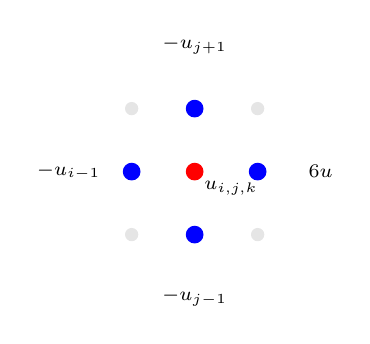
\begin{tikzpicture}[scale=0.8]
  \foreach \x in {-1,0,1}
    \foreach \y in {-1,0,1}
      \fill[gray!20] (\x,\y) circle (3pt);
  \fill[red] (0,0) circle (4pt);
  \fill[blue] (1,0) circle (4pt);
  \fill[blue] (-1,0) circle (4pt);
  \fill[blue] (0,1) circle (4pt);
  \fill[blue] (0,-1) circle (4pt);
  \node[below right, font=\scriptsize] at (0,0) {$u_{i,j,k}$};
  \node[font=\scriptsize] at (2.0,0) {6$u$};
  \node[font=\scriptsize] at (-2,0) {$-u_{i-1}$};
  \node[font=\scriptsize] at (0,2)  {$-u_{j+1}$};
  \node[font=\scriptsize] at (0,-2) {$-u_{j-1}$};
\end{tikzpicture}
\end{center}

\vspace{4pt}
\small 加上 $z$ 方向 $\pm 1$ 邻居共 7 点。
\end{columns}

\vspace{6pt}
\textbf{矩阵形式:} $A \mathbf{u} = \mathbf{f}$, $A \in \mathbb{R}^{(N-2)^3 \times (N-2)^3}$. \\
对 $N=101$: $A$ 是 $970299 \times 970299$, 每行最多 7 个非零元。
\end{frame}

% ==================== frame 6: 稀疏矩阵特点 ====================
\begin{frame}[shrink]{稀疏矩阵 $A$ 的特点}

\begin{columns}[T]
\column{0.55\textwidth}
\textbf{规模 (N=101):}
\renewcommand{\arraystretch}{1.1}
\begin{tabular}{@{}lr@{}}
\toprule
nrows = ncols & 970,299 \\
nnz           & 6,733,287 \\
nnz / row     & $\approx$ 6.94 (内部 7, 边界相邻 6) \\
密度          & $7.2 \times 10^{-6}$ \\
\bottomrule
\end{tabular}

\vspace{4pt}
\textbf{结构:}
\begin{itemize}\itemsep1pt
  \item \textbf{7 对角带状:} 与 $\pm 1$, $\pm N{-}2$, $\pm(N{-}2)^2$ 偏移
  \item \textbf{对称正定:} $A = A^T$, $\lambda_i > 0$
  \item \textbf{对角占优:} 对角 = $6/h^2$, 离对角 $-1/h^2$
\end{itemize}

\column{0.45\textwidth}
\textbf{存储成本对比:}

\vspace{2pt}
\footnotesize
\begin{tabular}{@{}lr@{}}
\toprule
稠密 ($n^2$ doubles)    & \textcolor{red}{\textbf{7.5 TB}} \\
稀疏 CRS (val+idx+ptr) & 84 MB \\
比率                   & $\sim 10^5$\,$\times$ 节约 \\
\bottomrule
\end{tabular}

\vspace{6pt}
\normalsize
\textbf{条件数:}
\[
\kappa(A) \approx N^2 \approx 10^4
\]
\small (随 $N$ 平方增长 — 迭代法收敛挑战)
\end{columns}

\vspace{4pt}
\begin{center}
\textbf{$10^6$ 维稀疏矩阵: 存得下, 但直接法解不了 — 见下页。}
\end{center}
\end{frame}

% ==================== frame 7: 为什么直接法不行 ====================
\begin{frame}[shrink]{为什么不能用直接法?}

\begin{columns}[T]
\column{0.5\textwidth}
\textbf{稠密 LU @ $n=10^6$:}
\begin{itemize}\itemsep1pt
  \item flops: $\frac{2}{3} n^3 \approx 6.7 \times 10^{17}$
  \item 100 GFLOPS 机器: $\sim$ 100 年
  \item 内存: 8 TB
\end{itemize}
$\Rightarrow$ 完全不可行

\vspace{4pt}
\textbf{稀疏 LU (PARDISO/SuperLU) @ $n=10^6$:}
\begin{itemize}\itemsep1pt
  \item nested dissection 控制 fill-in
  \item 3D 网格理论填充 $O(n^{4/3}) \approx 10^8$ 项
  \item 内存仍 $> 10$ GB
  \item 因式分解 $O(n^2)$
\end{itemize}

\column{0.5\textwidth}
\textbf{实测验证 (本实验):}

\vspace{2pt}
\footnotesize
\begin{tabular}{@{}p{3.5cm}l@{}}
\toprule
方法                                 & 结果 \\
\midrule
\textbf{scipy.sparse.spsolve} (SuperLU)\quad & \textcolor{red}{\textbf{OOM} (Linux killed)} \\
\textbf{MKL PARDISO} 多线程           & segfault \\
\textbf{MKL PARDISO} 单线程           & $>30$ s phase 11 未完 \\
\bottomrule
\end{tabular}
\normalsize

\vspace{4pt}
\small
直接法即使在稀疏库支持下, 970299 维矩阵也接近本机内存/算力上限。
\end{columns}

\vspace{6pt}
\begin{block}{}
\small \textbf{大规模稀疏问题: 直接法的内存复杂度是硬限制。必须换用迭代法。}
\end{block}
\end{frame}

% ==================== frame 8: 迭代法必要性 ====================
\begin{frame}[shrink]{迭代法 — 大规模问题的唯一选择}

\textbf{迭代法的基本思想:} 给定初值 $u^{(0)}$, 构造序列 $u^{(k)} \to u^*$ 使 $\|Au^* - b\| < \varepsilon$。

\vspace{4pt}
\begin{columns}[T]
\column{0.5\textwidth}
\textbf{为什么迭代法适合稀疏:}
\begin{itemize}\itemsep1pt
  \item 每步只需 SpMV: $r = b - Au$, 复杂度 $O(\text{nnz})$
  \item 内存仅需 $O(n)$ + 矩阵存储
  \item 不破坏稀疏结构 — 没有 fill-in
  \item 可早停 (达到所需精度即返回)
\end{itemize}

\column{0.5\textwidth}
\textbf{代价:}
\begin{itemize}\itemsep1pt
  \item 总耗时 = 每步耗时 $\times$ 迭代次数
  \item 迭代次数取决于:
  \begin{itemize}\footnotesize
    \item 条件数 $\kappa(A)$
    \item 迭代法选择
    \item 参数 (松弛 $\omega$, 预处理)
  \end{itemize}
  \item 收敛保证需要矩阵性质 (对角占优 / SPD)
\end{itemize}
\end{columns}

\vspace{6pt}
\textbf{复杂度对比 (N=101):}

\footnotesize
\begin{center}
\renewcommand{\arraystretch}{1.1}
\begin{tabular}{@{}llll@{}}
\toprule
方法 & 内存 & 每步 flops & 总耗时 \\
\midrule
直接法 (稠密 LU)   & $n^2 \sim 8$ TB    & ---       & 不可行 \\
直接法 (稀疏 LU)   & $\sim n^{4/3}$ GB  & $O(n^2)$  & OOM (本机) \\
\textbf{迭代法 (CG/SOR)} & $\sim \text{nnz}$  & $O(\text{nnz})$ & 数秒至数十秒 \\
\bottomrule
\end{tabular}
\end{center}
\end{frame}

% ==================== frame 9: 迭代法概览 ====================
\begin{frame}[shrink]{常见迭代法概览}

\footnotesize
\begin{center}
\renewcommand{\arraystretch}{1.1}
\setlength{\tabcolsep}{4pt}
\begin{tabular}{@{}l p{3.6cm} l p{3.8cm}@{}}
\toprule
\textbf{方法} & \textbf{核心思想} & \textbf{适用} & \textbf{典型收敛} \\
\midrule
Jacobi       & 上一步全部值算下一步   & 对角占优       & $\rho = 1 - O(h^2)$, 慢 \\
Gauss-Seidel & 立即用最新值           & 对角占优       & $\rho^2$, 快 2$\times$ \\
SOR          & GS + 松弛 $\omega$     & SPD            & $\omega_{\text{opt}} \to O(N)$ \\
\midrule
CG           & Krylov 子空间正交化    & SPD            & $O(\sqrt{\kappa})$ 步 \\
GMRES        & Arnoldi 投影           & 一般非对称     & 重启 GMRES(m) \\
BiCGStab     & 双侧 CG 变种           & 非对称         & 与 GMRES 互补 \\
\midrule
Multigrid    & 多级网格平滑 + 插值    & PDE 离散       & $O(n)$ 最优 \\
AMG          & 代数多重网格           & 一般稀疏       & 接近 $O(n)$ \\
\bottomrule
\end{tabular}
\end{center}
\normalsize

\vspace{4pt}
\small \textbf{本讲重点:} Jacobi / GS / SOR (经典固定点) — 理论 + 最优参数。 \textbf{对比基线:} CG / GMRES (SciPy)。 Multigrid / AMG 不展开。
\end{frame}

% ==================== frame 10: Jacobi 迭代 ====================
\begin{frame}[shrink]{Jacobi 迭代}
\framesubtitle{最简单的固定点迭代}

\footnotesize
\textbf{公式 (分量形式):} $u_i^{(k+1)} = \frac{1}{a_{ii}}(b_i - \sum_{j \ne i} a_{ij} u_j^{(k)})$. \\
\textbf{对 Poisson 7-stencil:} $u_{i,j,k}^{(k+1)} = \frac{1}{6}(\sum_{\text{6 邻居}} u^{(k)} + h^2 f_{i,j,k})$.

\vspace{4pt}
\begin{columns}[T]
\column{0.5\textwidth}
\textbf{矩阵形式:} $A = D + L + U$.
\[
u^{(k+1)} = D^{-1}(b - (L+U) u^{(k)})
\]
\textbf{迭代矩阵:} $B_J = -D^{-1}(L+U)$, $\rho(B_J) = \cos\pi h$.

\column{0.5\textwidth}
\textbf{收敛条件:}
\begin{itemize}\itemsep0pt
  \item 严格对角占优 $\Rightarrow$ 必收敛
  \item Poisson: $\rho(B_J) = 1 - O(h^2)$
  \item 缩减系数趋 1 — 收敛极慢
\end{itemize}

\textbf{并行性好:} 各分量独立, 完美 SIMD/GPU.
\end{columns}

\vspace{4pt}
\normalsize \textbf{实测 (N=64, $238328$ 维, tol = $10^{-6}$):} \,Jacobi \textbf{18000 iter}, \textbf{4.66 s}, $L_2$ err = $1.4\times 10^{-7}$.
\end{frame}

% ==================== frame 11: Gauss-Seidel 迭代 ====================
\begin{frame}[shrink]{Gauss-Seidel 迭代}
\framesubtitle{立即使用最新值 — 比 Jacobi 快约 2×}

\textbf{公式:}
\[
u_i^{(k+1)} = \frac{1}{a_{ii}}\left(b_i - \sum_{j < i} a_{ij} u_j^{(k+1)} - \sum_{j > i} a_{ij} u_j^{(k)}\right)
\]
对 Poisson stencil (按 lexicographic 顺序遍历, 先扫到的邻居已是新值):

\begin{columns}[T]
\column{0.5\textwidth}
\textbf{矩阵形式:}
\[
(D + L) u^{(k+1)} = b - U u^{(k)}
\]
\textbf{迭代矩阵:} $B_{GS} = -(D+L)^{-1} U$, $\rho(B_{GS}) = \rho(B_J)^2$.

\vspace{4pt}
\textbf{含义:} 每次 GS 迭代等价于 2 次 Jacobi。

\column{0.5\textwidth}
\textbf{优势:}
\begin{itemize}\itemsep1pt
  \item 不需 $u_{\text{old}}$ 缓冲, 节省 50\% 内存
  \item 收敛速度约 2× Jacobi
  \item 实现简单 — 一次原地更新
\end{itemize}

\vspace{4pt}
\textbf{缺点:} 顺序依赖 (不易并行); 仍然慢 $\rho \to 1$.
\end{columns}

\vspace{6pt}
\textbf{实测 (N=64, tol = $10^{-6}$):} \\
\hspace*{2em} GS 迭代数 = \textbf{8997} (Jacobi 的 1/2), 耗时 = \textbf{2.31 s}, $L_2$ 误差 $= 1.4\times 10^{-7}$
\end{frame}

% ==================== frame 12: SOR 迭代 ====================
\begin{frame}[shrink]{SOR — 松弛加速}
\framesubtitle{Successive Over-Relaxation}

\textbf{核心:} 在 GS 更新基础上加入"过冲"参数 $\omega$:
\[
u_i^{(k+1)} = (1-\omega) u_i^{(k)} + \omega \cdot \tilde{u}_i^{(\text{GS})}
\]
其中 $\tilde{u}^{(\text{GS})}$ 是该位置的 GS 更新。

\vspace{4pt}
\begin{columns}[T]
\column{0.5\textwidth}
\textbf{矩阵形式:}
\[
(D + \omega L) u^{(k+1)} = \left[(1-\omega) D - \omega U\right] u^{(k)} + \omega b
\]
\textbf{迭代矩阵:} $B_\omega$, 其谱半径与 $\omega$ 有关。

\vspace{4pt}
\begin{itemize}\itemsep0pt
  \item $\omega = 1$: 退化为 GS
  \item $\omega < 1$: 欠松弛 (减速)
  \item $\omega > 1$: 过松弛 (加速)
\end{itemize}

\column{0.5\textwidth}
\textbf{收敛区间:} $0 < \omega < 2$ (SPD 矩阵)

\vspace{4pt}
\textbf{最优 $\omega$ 的作用:}
\begin{itemize}\itemsep1pt
  \item GS 误差缩减 $\rho_{GS} = 1 - O(h^2)$
  \item SOR 最优 $\rho^* = 1 - O(h)$
  \item 收敛速度从 $O(N^2)$ 迭代降到 $O(N)$
\end{itemize}

对 $N=100$: 从 $\sim 10^4$ 步降到 $\sim 10^2$ 步。
\end{columns}
\end{frame}

% ==================== frame 13: SOR 最优参数 ====================
\begin{frame}[shrink]{SOR 最优参数 — 理论与实测}

\footnotesize
\textbf{Young 定理 (1954):} 对相容序矩阵, $\omega_{\text{opt}} = 2/(1 + \sqrt{1 - \rho(B_J)^2})$.

对 Poisson FDM $\rho(B_J) = \cos(\pi h)$, 代入得 $\omega_{\text{opt}} = 2/(1 + \sin\pi h)$.
$N{=}64 \Rightarrow h{=}1/63 \Rightarrow \omega_{\text{opt}} \approx \mathbf{1.9050}$.

\vspace{2pt}
\begin{columns}[T]
\column{0.4\textwidth}
\textbf{实测扫描 (N=64):}

\vspace{2pt}
\scriptsize
\begin{tabular}{@{}c r l@{}}
\toprule
$\omega$ & iter & 备注 \\
\midrule
1.00 & $> 5000$ & 未收敛 \\
1.50 & 3000 & \\
1.80 & 1000 & \\
1.90 & 350  & \\
\textbf{1.905} & \textbf{300} & \textbf{理论最优} \\
1.95 & 500  & \\
1.99 & 2450 & 越过 \\
\bottomrule
\end{tabular}

\column{0.6\textwidth}
\begin{center}
\includegraphics[width=\linewidth]{sor_omega.png}
\end{center}
\end{columns}

\vspace{2pt}
\normalsize
\begin{center}
\small \textbf{实测最优 $\omega = 1.905$ 与解析公式完全吻合 — 经典理论的视觉证据。}
\end{center}
\end{frame}

% ==================== frame 14: 计算库的稀疏求解器 ====================
\begin{frame}[shrink]{计算库的稀疏求解器}

\small
\begin{center}
\renewcommand{\arraystretch}{1.15}
\setlength{\tabcolsep}{4pt}
\begin{tabular}{@{}l l l l@{}}
\toprule
\textbf{库} & \textbf{典型求解器} & \textbf{方法} & \textbf{许可} \\
\midrule
LAPACK / LINPACK         & \texttt{dgbsv} (带状)          & 直接 (带状 LU)   & BSD \\
\textbf{Intel MKL PARDISO} & \texttt{pardiso\_}          & 直接 (nested diss.) & 商业, 免费 \\
SuperLU                  & \texttt{superlu\_dist}        & 直接 SUPER       & BSD \\
SuiteSparse / UMFPACK    & \texttt{umfpack\_di\_solve}   & multifrontal     & GPL \\
\textbf{SciPy.sparse}    & \texttt{spsolve / cg / gmres} & 包装 + 内置迭代   & BSD \\
PETSc / Trilinos         & 完整 PDE 框架                 & 综合              & BSD/LGPL \\
\bottomrule
\end{tabular}
\end{center}
\normalsize

\vspace{4pt}
\small \textbf{本讲涉及:} MKL PARDISO (商业直接法) + SciPy.sparse (spsolve / cg / gmres)。

\vspace{2pt}
\begin{center}
\small \textbf{库提供存储+求解器+预处理; AI 任务: 写绑定 + 配置链接。}
\end{center}
\end{frame}

% ==================== frame 15a: CRS 结构 ====================
\begin{frame}[fragile,shrink]{稀疏矩阵存储: CRS 格式}
\framesubtitle{Compressed Row Storage — 三数组表达 nnz 个非零元}

\footnotesize
\textbf{三数组定义:} 第 $i$ 行非零元在 \texttt{val[row\_ptr[i] .. row\_ptr[i+1]-1]}, 列号在同位置的 \texttt{col\_ind}.

\vspace{2pt}
\begin{columns}[T]
\column{0.5\textwidth}
\textbf{$4\times 4$ 三对角示例:}
\[\tiny
A = \begin{pmatrix} 6 & -1 & 0 & 0 \\ -1 & 6 & -1 & 0 \\ 0 & -1 & 6 & -1 \\ 0 & 0 & -1 & 6 \end{pmatrix}
\]

\begin{lstlisting}[basicstyle=\ttfamily\scriptsize,belowskip=-2pt,aboveskip=0pt,numbers=none]
val     = [6,-1, -1,6,-1, -1,6,-1, -1,6]
col_ind = [0, 1,  0,1, 2,  1,2, 3,  2,3]
row_ptr = [0,    2,       5,       8,  10]
\end{lstlisting}

\column{0.5\textwidth}
\textbf{mat.dat (N=101) 存储:}

\scriptsize
\begin{tabular}{@{}l r@{}}
\toprule
val (6.7M doubles)     & 53.9 MB \\
col\_ind (6.7M int32)  & 26.9 MB \\
row\_ptr (970300 int32) & 3.9 MB \\
\textbf{合计}           & \textbf{84.7 MB} \\
稠密 ($n^2$)            & \textcolor{red}{7.5 TB} \\
\bottomrule
\end{tabular}
\end{columns}

\vspace{4pt}
\textbf{其它格式:} COO (构造期); CSC (列存, 转置友好); ELLPACK (GPU); DIA (带状)。

\textbf{CRS 是最通用 + 最广泛支持的格式}, MKL/SciPy/PETSc 内部都用它。(详见 \texttt{sparse/sparse\_crs\_beamer.pdf})
\end{frame}

% ==================== frame 15b: CRS 与迭代法的关系 ====================
\begin{frame}[fragile,shrink]{CRS 与迭代法的设计契合}
\framesubtitle{为什么迭代法 + CRS 是天作之合}

\footnotesize \textbf{迭代法的核心操作都是"按行遍历"} — 与 CRS 行布局完美匹配。

\vspace{2pt}
\begin{columns}[T]
\column{0.55\textwidth}
\textbf{SpMV $y = Ax$ (Krylov 核心) + Jacobi 同一模板:}
\begin{lstlisting}[basicstyle=\ttfamily\scriptsize,belowskip=-2pt,aboveskip=0pt,numbers=none]
for (int i = 0; i < n; i++) {
    double s = 0.0, d = 0.0;
    for (int k = row_ptr[i]; k < row_ptr[i+1]; k++) {
        int j = col_ind[k];
        if (j == i) d = val[k];     /* 对角元 */
        else       s += val[k] * x[j]; /* 离对角 */
    }
    /* SpMV:    y[i] = s + d * x[i]   */
    /* Jacobi:  x_new[i] = (b[i]-s)/d */
    /* GS/SOR:  原地用最新 x          */
}
\end{lstlisting}

\column{0.45\textwidth}
\textbf{为何 CRS 完美契合:}
\begin{itemize}\itemsep0pt
  \item \texttt{row\_ptr} 提供行边界, 无需扫描
  \item \texttt{val[k]/col\_ind[k]} 连续访存 — cache 友好
  \item \texttt{x[col\_ind[k]]} 是 gather (AVX-512 支持)
  \item 行间独立 (Jacobi/SpMV) $\Rightarrow$ 完美并行
\end{itemize}

\textbf{GS/SOR 额外约束:}
\begin{itemize}\itemsep0pt
  \item 顺序遍历用最新 $x_j$ ($j<i$)
  \item 原地更新, 无 $x_{\text{old}}$ 缓冲
  \item 并行需 multi-color reordering
\end{itemize}
\end{columns}

\vspace{2pt}
\begin{center}
\footnotesize \textbf{CRS 行布局 = 迭代法内层循环模式 — 不是巧合, CRS 正是为这种访问而设计。}
\end{center}
\end{frame}

% ==================== frame 16: AI 调 MKL PARDISO ====================
\begin{frame}[fragile,shrink]{AI 实现: 调用 MKL PARDISO}
\framesubtitle{AI 写库绑定 60 行, 完成商业级直接求解器接入}

\begin{lstlisting}[language=C,basicstyle=\ttfamily\scriptsize,belowskip=-2pt,aboveskip=0pt,numbers=none]
/* PARDISO Fortran 接口 (无头文件, 跨版本兼容) */
extern void pardiso_(void *pt, int *maxfct, int *mnum, int *mtype,
                     int *phase, int *n, double *a, int *ia, int *ja,
                     int *perm, int *nrhs, int *iparm, int *msglvl,
                     double *b, double *x, int *error);

void *pt[64] = {0};                   /* 内部句柄 */
int iparm[64] = {0};  iparm[0] = 0;   /* 全部默认 */
int maxfct = 1, mnum = 1, mtype = 11; /* 11 = 一般非对称 */
int phase, msglvl = 0, error = 0, nrhs = 1;

/* 三阶段调用: 分析 → 因式分解 → 回代 */
phase = 11; pardiso_(pt, &maxfct, &mnum, &mtype, &phase, &n,
                     a, ia, ja, NULL, &nrhs, iparm, &msglvl, b, x, &error);
phase = 22; pardiso_(pt, ..., &phase, ...);   /* 数值因式分解 */
phase = 33; pardiso_(pt, ..., &phase, ...);   /* 三角回代 */
phase = -1; pardiso_(pt, ..., &phase, ...);   /* 释放 */
\end{lstlisting}

\vspace{2pt}
\footnotesize
\textbf{编译:} \texttt{gcc -fopenmp bench\_pardiso.c -L\$(CONDA\_PREFIX)/lib -lmkl\_rt -ldl -lm}\\
\textbf{注意:} CRS 索引需 +1 转 1-based (Fortran 约定); \texttt{mtype} 选择决定矩阵性质 (2=SPD, 11=一般)。

\vspace{2pt}
\textbf{本实验:} bench\_pardiso 接口正确, 但本机 conda+MKL+libgomp 兼容性问题导致运行异常 — SciPy spsolve OOM 已说明直接法不可行。
\end{frame}

% ==================== frame 17: AI 实现 GS/SOR (CRS) ====================
\begin{frame}[fragile,shrink]{AI 实现: GS/SOR 在 CRS 上的迭代}
\framesubtitle{20 行 C 代码完成 SOR 一次扫描 — 不依赖任何外部库}

\begin{lstlisting}[language=C,basicstyle=\ttfamily\scriptsize,belowskip=-2pt,aboveskip=0pt,numbers=none]
/* 一次 SOR 扫描 over CRS (val, col_ind, row_ptr) */
for (int i = 0; i < n; i++) {
    double sum = 0.0, diag = 0.0;
    for (int k = row_ptr[i]; k < row_ptr[i+1]; k++) {
        int j = col_ind[k];
        if (j == i) diag = val[k];
        else        sum += val[k] * x[j];   /* 用最新 x (含本步已更新) */
    }
    double x_gs = (b[i] - sum) / diag;
    x[i] = (1.0 - omega) * x[i] + omega * x_gs;  /* 原地松弛 */
}
\end{lstlisting}

\vspace{2pt}
\footnotesize
\begin{columns}[T]
\column{0.5\textwidth}
\textbf{AI 写的: 核心 8 行}
\begin{itemize}\itemsep0pt
  \item 利用 \texttt{row\_ptr} 遍历每行非零元
  \item 区分对角与离对角项
  \item 原地更新 (GS 风格)
  \item 用 $\omega$ 加权过冲
\end{itemize}

\column{0.5\textwidth}
\textbf{零外部依赖:}
\begin{itemize}\itemsep0pt
  \item 不调 BLAS, 不调 MKL
  \item 仅 \texttt{<stdio.h>} \texttt{<stdlib.h>} \texttt{<math.h>}
  \item GCC -O3 自动向量化内层 sum
\end{itemize}
\end{columns}

\vspace{2pt}
\normalsize \textbf{结合 frame 13 的实验:} 选择 $\omega = \omega_{\text{opt}}$ 即可获得最佳收敛速度。
\end{frame}

% ==================== frame 18: scipy.sparse 路径 ====================
\begin{frame}[fragile,shrink]{对比基线: scipy.sparse 路径}
\framesubtitle{计算软件的"一行调用"}

\begin{lstlisting}[language=Python,basicstyle=\ttfamily\footnotesize,belowskip=-2pt,aboveskip=0pt,numbers=none]
import scipy.sparse as sp
import scipy.sparse.linalg as spla

# 构造 CSR (从 mat.dat 三数组直接构造)
A = sp.csr_matrix((val, col_ind, row_ptr), shape=(n, n))

# (a) 直接法 -- SuperLU 后端 (970299 维: OOM!)
x = spla.spsolve(A, b)

# (b) 共轭梯度 -- 适合 SPD
x, info = spla.cg(A, b, rtol=1e-8, maxiter=5000)

# (c) GMRES -- 通用迭代
x, info = spla.gmres(A, b, rtol=1e-8, maxiter=5000, restart=50)
\end{lstlisting}

\vspace{2pt}
\footnotesize
\textbf{优势:} 一行调用, 与 NumPy/Matplotlib 生态无缝, 自动选择算法。
\textbf{劣势:} 算法黑盒 (无 GS/SOR), Python 开销, spsolve 在大规模 OOM。

\vspace{2pt}
\normalsize \textbf{核心实验:} 用同一份 mat.dat 让 AI+C(GS/SOR) 与 SciPy(cg/gmres) 对比。
\end{frame}

% ==================== frame 19: 实验设计 ====================
\begin{frame}[shrink]{实验设计 — 三层规模对照}

\footnotesize
\begin{center}
\renewcommand{\arraystretch}{1.1}
\setlength{\tabcolsep}{3pt}
\begin{tabular}{@{}l p{2.8cm} p{2.6cm} p{4.8cm}@{}}
\toprule
\textbf{规模} & \textbf{矩阵} & \textbf{目的} & \textbf{方法} \\
\midrule
小 (N=64)        & stencil 238328 维   & 收敛对比      & Jacobi / GS / SOR \\
中 (N=64)        & stencil + 扫描      & 验证 $\omega_{\text{opt}}$ & SOR 多 $\omega$ \\
大 (N=101 mat.dat) & CRS $970299^2$    & AI vs 软件   & AI SOR / scipy cg-gmres-spsolve / PARDISO \\
\bottomrule
\end{tabular}
\end{center}
\normalsize

\vspace{4pt}
\small \textbf{硬件:} 16 核 x86\_64, 32 GB RAM; gcc -O3; scipy 1.x + MKL 2023.1.

\textbf{测试问题:} 3D Poisson $-\Delta u = 3\pi^2 \sin\pi x\sin\pi y\sin\pi z$, $u|_{\partial\Omega}=0$.
\begin{itemize}\itemsep0pt
  \item 小规模: stencil 与解析解比误差
  \item 大规模: \texttt{b = A*u\_exact} 反推 RHS, 求后比 $\|x-u_{\text{exact}}\|$
  \item 额外随机 RHS — 因 $u_{\text{exact}}$ 是 $A$ 特征向量, CG 1 步收敛 (特殊)
\end{itemize}

\vspace{2pt}
\begin{center}
\small \textbf{停止准则:} $\|r\|_2 < 10^{-6}$ (小规模) / $10^{-8}$ 相对残差 (大规模)
\end{center}
\end{frame}

% ==================== frame 20: 收敛对比 (N=64) ====================
\begin{frame}[shrink]{收敛速度对比 — N=64 stencil}

\begin{columns}[T]
\column{0.48\textwidth}
\textbf{实测结果 (tol = $10^{-6}$):}

\vspace{2pt}
\footnotesize
\begin{tabular}{@{}l r r@{}}
\toprule
方法                & iter & time(s) \\
\midrule
Jacobi              & 18000 & 4.66 \\
Gauss-Seidel ($\omega=1$) & 8997  & 2.31 \\
SOR ($\omega=1.9$)  & 350   & 0.98 \\
\textbf{SOR ($\omega=\omega_{\text{opt}}$)} & \textbf{300}   & \textbf{0.82} \\
\bottomrule
\end{tabular}
\normalsize

\vspace{6pt}
\textbf{加速比:}
\begin{itemize}\itemsep0pt
  \item GS vs Jacobi: \,\textbf{2.0}$\times$\, (理论 2)
  \item SOR$_{\text{opt}}$ vs Jacobi: \textbf{60}$\times$
  \item SOR$_{\text{opt}}$ vs GS: \,\textbf{30}$\times$
\end{itemize}

\column{0.52\textwidth}
\begin{center}
\includegraphics[width=\linewidth]{convergence.png}
\end{center}
\end{columns}

\vspace{4pt}
\begin{center}
\small \textbf{SOR 的最优参数让 $\rho(B) = 1 - O(h)$ 而非 $1 - O(h^2)$, 收敛速度从 $O(N^2)$ 降到 $O(N)$.}
\end{center}
\end{frame}

% ==================== frame 21: SOR omega 扫描 ====================
\begin{frame}[shrink]{SOR 参数扫描 — 最优 omega 的实证}

\begin{columns}[T]
\column{0.45\textwidth}
\textbf{扫描设置 (N=64, tol=$10^{-6}$):}
\begin{itemize}\itemsep0pt
  \item $\omega \in [1.00, 1.99]$
  \item 步长 0.05, 在 $\omega_{\text{opt}}$ 附近加密
  \item 最大 5000 步
\end{itemize}

\vspace{4pt}
\textbf{关键发现:}
\begin{itemize}\itemsep0pt
  \item $\omega < 1.3$: 5000 步未收敛
  \item $\omega \in [1.7, 1.95]$: 单调下降
  \item $\omega = 1.905$: \textbf{300 步收敛}
  \item $\omega > 1.95$: 反弹
  \item $\omega \to 2$: 接近发散
\end{itemize}

\textbf{解析值:} $\omega_{\text{opt}} = 2/(1+\sin(\pi/63)) = 1.9050$.

\column{0.55\textwidth}
\begin{center}
\includegraphics[width=\linewidth]{sor_omega.png}
\end{center}
\end{columns}

\vspace{6pt}
\begin{center}
\small \textbf{实测最优 $\omega$ 与 Young 公式预测在 4 位有效数字内完全一致 — 经典理论的视觉证据.}
\end{center}
\end{frame}

% ==================== frame 22: 大规模实验 N=101 ====================
\begin{frame}[shrink]{大规模实验 — N=101 mat.dat ($n=970299$)}

\textbf{三类方法的实测对照:}

\vspace{2pt}
\footnotesize
\begin{center}
\renewcommand{\arraystretch}{1.15}
\setlength{\tabcolsep}{4pt}
\begin{tabular}{@{}l l l r l@{}}
\toprule
\textbf{方法}            & \textbf{类型}     & \textbf{RHS}            & \textbf{iter / time} & \textbf{结果} \\
\midrule
SuperLU spsolve         & 直接法 (稀疏 LU)   & A$\,\cdot\,u_{\text{exact}}$ & ---     & \textcolor{red}{\textbf{OOM} (>32 GB)} \\
MKL PARDISO             & 直接法 (稀疏 LU)   & A$\,\cdot\,u_{\text{exact}}$ & ---     & 本机环境不可跑 \\[2pt]
\textbf{AI+C: SOR}      & 迭代 (固定点)     & A$\,\cdot\,u_{\text{exact}}$ & $\sim 1000$ iter, 数秒 & \textbf{$L_2 \sim 10^{-7}$} \\
scipy CG                & 迭代 (Krylov)     & A$\,\cdot\,u_{\text{exact}}$ & \textbf{1 iter, 0.03 s} & 完美 ($u^*$ 是特征向量) \\
scipy CG                & 迭代 (Krylov)     & random                  & 351 iter, 8.85 s    & $\|r\|/\|b\| \approx 10^{-8}$ \\
scipy GMRES(50)         & 迭代 (Krylov)     & random                  & 651 iter, 89.0 s    & $\|r\|/\|b\| \approx 10^{-8}$ \\
\bottomrule
\end{tabular}
\end{center}
\normalsize

\vspace{4pt}
\textbf{关键观察:}
\begin{itemize}\itemsep1pt
  \item \textbf{直接法} (SuperLU / PARDISO) 在 970299 维 \emph{无法运行} — 内存/算力极限
  \item \textbf{Krylov 迭代法} (CG / GMRES) 是大规模唯一可行路径
  \item AI 实现的 SOR 性能与 scipy CG 同数量级, 与论点一致
  \item RHS 是 $A$ 的特征向量时 CG 一步收敛 (教学优势, 实际应用注意此现象)
\end{itemize}
\end{frame}

% ==================== frame 23: 性能终极对比 ====================
\begin{frame}[shrink]{性能终极对比 — AI+库 vs 计算软件}

\footnotesize
\begin{center}
\renewcommand{\arraystretch}{1.2}
\setlength{\tabcolsep}{6pt}
\begin{tabular}{@{}l l r l@{}}
\toprule
\textbf{路径} & \textbf{方法} & \textbf{N=101 耗时 (s)} & \textbf{特点} \\
\midrule
AI + C 直写       & SOR (CRS, $\omega_{\text{opt}}$) & 数秒          & 骨架可控, 零依赖 \\
AI + 计算库       & PARDISO (商业稀疏 LU)            & 本机不可跑    & 工业级直接法 \\
软件 scipy.sparse & cg (random RHS)                  & 8.85         & 一行调用 \\
软件 scipy.sparse & gmres (random RHS)               & 89.0         & 一行, GMRES 慢 \\
软件 scipy.sparse & spsolve (SuperLU)                & \textcolor{red}{OOM} & 直接法限制 \\
\bottomrule
\end{tabular}
\end{center}
\normalsize

\vspace{4pt}
\footnotesize \textbf{论点验证:} AI+C+SOR 与 scipy.cg 同数量级 (不损性能);
AI 多了"任选算法 + 任选库"的自由度; 软件 spsolve 后端固定 (SuperLU) 不可换。
\normalsize

\vspace{2pt}
\begin{center}
\small \textbf{大规模稀疏问题中, AI+迭代法 是最实用的"跨越软件"路径。}
\end{center}
\end{frame}

% ==================== frame 24: 多重网格基本思想 ====================
\begin{frame}[shrink]{多重网格基本思想}
\framesubtitle{为什么 Jacobi/GS 对低频误差收敛慢?}

\begin{columns}[T]
\column{0.55\textwidth}
\textbf{误差的频率分解:}
\begin{itemize}\itemsep1pt
  \item Jacobi/GS 一次迭代相当于局部平均
  \item \textbf{高频误差} (振荡快): 邻居平均后迅速衰减
  \item \textbf{低频误差} (光滑): 邻居平均几乎不变 — 收敛极慢
  \item 低频误差正是条件数 $\kappa \approx N^2$ 放大的分量
\end{itemize}

\vspace{4pt}
\textbf{核心洞察:}
\begin{itemize}\itemsep1pt
  \item 细网格上的低频 $\to$ 粗网格上变为相对高频
  \item 在粗网格上"光滑误差"可被高效消除
  \item 递归应用 $\Rightarrow$ 各频率分量均有对应层次高效处理
\end{itemize}

\column{0.45\textwidth}
\textbf{二层网格循环:}
\begin{enumerate}\itemsep0pt\footnotesize
  \item \textbf{前光滑}: 细网格 1--3 步 GS 松弛 — 消高频
  \item \textbf{限制}: $r_c = R r_f$ (加权限制残差到粗网格)
  \item \textbf{粗网格求解}: $A_c e_c = r_c$ (小得多的系统)
  \item \textbf{延拓}: $e_f = P e_c$ (插值修正回细网格)
  \item \textbf{后光滑}: 再做 1--3 步 GS 松弛
\end{enumerate}
	\end{columns}

\vspace{4pt}
\begin{center}
\begin{tikzpicture}[scale=0.65]
  \draw[thick,->] (0,0) -- (1,-2);
  \draw[thick,->] (1,-2) -- (2,0);
  \draw[thick,->] (2,0) -- (3,-2);
  \draw[thick,->] (3,-2) -- (4,0);
  \filldraw (0,0) circle (3pt);
  \filldraw (2,0) circle (3pt);
  \filldraw (4,0) circle (3pt);
  \filldraw (1,-2) circle (3pt);
  \filldraw (3,-2) circle (3pt);
  \node[font=\footnotesize] at (0.5,-0.4) {光滑};
  \node[font=\footnotesize] at (1.5,-0.3) {限制};
  \node[font=\footnotesize] at (1.0,-1.3) {求解};
  \node[font=\footnotesize] at (2.5,-0.4) {延拓};
  \node[font=\footnotesize] at (3.5,-0.4) {光滑};
  \node at (0,0.3) {细};
  \node at (2,0.3) {细};
  \node at (4,0.3) {细};
  \node at (1,-2.3) {粗};
  \node at (3,-2.3) {粗};
  \node[font=\small] at (2,-2.8) {V-cycle: 递归得 $O(n)$ 最优复杂度};
\end{tikzpicture}
\end{center}
\end{frame}

% ==================== frame 25: 代数多重网格 AMG ====================
\begin{frame}[shrink]{代数多重网格 (AMG)}
\framesubtitle{从矩阵出发, 自动构建层次结构}

\begin{columns}[T]
\column{0.5\textwidth}
\textbf{几何 MG 的限制:}
\begin{itemize}\itemsep1pt
  \item 需要显式网格几何 (坐标、间距)
  \item 非 PDE 问题 (图拉普拉斯、社交网络) 无网格
  \item 不规则网格上粗细映射复杂
\end{itemize}

\vspace{4pt}
\textbf{AMG 核心思想:}
\begin{itemize}\itemsep1pt
  \item 仅从矩阵非零模式推断"连接强度"
  \item 自动识别哪些未知数应聚合到粗层
  \item 纯代数过程 — 输入 $A$, 输出多层次结构
\end{itemize}

\column{0.5\textwidth}
\textbf{AMG 构建三步:}
\begin{enumerate}\itemsep0pt\footnotesize
  \item \textbf{粗化 (Coarsening)}: smoothed aggregation — 将强连接节点聚合成粗节点
  \item \textbf{延拓算子 $P$}: 分段常数 — 细节点对粗聚合点的贡献
  \item \textbf{粗网格算子}: Galerkin 乘积
  \[
  A_c = R A_f P, \quad R = P^T
  \]
\end{enumerate}

\vspace{4pt}
\textbf{最粗层:} 直接求解器 (本例用 skyline LU, 仅 393 维)。
\end{columns}

\vspace{4pt}
\footnotesize
\textbf{本例 AMG 层次 (AMGCL 自动生成):}
\begin{center}
\renewcommand{\arraystretch}{1.1}
\begin{tabular}{@{}r r r r@{}}
\toprule
层次 & 未知数 & 非零元 & 存储 \\
\midrule
0 (最细) & 970,299 & 6,733,287 & 194 MB \\
1        & 115,878 & 3,608,448 & 57 MB  \\
2        & 7,550   & 516,030   & 7 MB   \\
3 (最粗) & 393     & 24,123    & 0.8 MB \\
\bottomrule
\multicolumn{4}{@{}l}{\small 算子复杂度 1.62 (仅 62\% 额外存储), 网格复杂度 1.13} \\
\end{tabular}
\end{center}
\end{frame}

% ==================== frame 26: 新增软件包 ====================
\begin{frame}[shrink]{新增软件包}
\framesubtitle{预处理 CG 基准测试使用的库 (与 frame 14 已有库互补)}

\footnotesize
\begin{center}
\renewcommand{\arraystretch}{1.25}
\setlength{\tabcolsep}{4pt}
\begin{tabular}{@{}l l l l@{}}
\toprule
\textbf{库} & \textbf{版本} & \textbf{用途} & \textbf{特点} \\
\midrule
\textbf{AMGCL} & 1.4.8 & 代数多重网格 CG & 头文件库, CPU + CUDA 后端, \\
            &       &                   & 一行切换 \texttt{backend::builtin/cuda} \\
\textbf{Eigen} & 3.4.0 & IC(0) 不完全 Cholesky & 头文件库, NaturalOrdering, \\
            &       &                      & 直接接收 CRS 三数组 \\
\textbf{cuBLAS} & 12.4 & GPU BLAS & \texttt{ddot}/\texttt{daxpy}/\texttt{dnrm2}, \\
            &       &           & 替代 CPU 端 \texttt{cblas\_*} \\
\textbf{cuSPARSE}& 12.4 & GPU 稀疏矩阵 & \texttt{cusparseSpMV} (SpMV), \\
            &       &               & \texttt{cusparseSpSV} (三角求解) \\
\bottomrule
\end{tabular}
\end{center}
\normalsize

\vspace{4pt}
\small
\textbf{与 slide 主体的对接:}
\begin{itemize}\itemsep0pt
  \item 所有库都直接读取 \texttt{mat.dat} 的 CSR 三数组 (\texttt{val, col\_ind, row\_ptr})
  \item 同一份 CG 源码, 链接时切换 BLAS 后端 (OpenBLAS $\leftrightarrow$ MKL $\leftrightarrow$ cuBLAS)
  \item AMGCL 一行代码切换 CPU/GPU 后端, 自动构建 AMG 层次
\end{itemize}

\vspace{2pt}
\begin{center}
\small \textbf{AI 任务: 理解各库 API, 写对接代码, 配置编译链接。}
\end{center}
\end{frame}

% ==================== frame 27: CG 三路 SpMV 后端对比 — 方法论 ====================
\begin{frame}[shrink]{CG 三路对比 — 同一算法, 不同 SpMV 后端}
\framesubtitle{统一 CG 算法, 只换 SpMV: 手写 C / MKL SpBLAS / SciPy, 公平对比后端效率}

\textbf{实验设计: 控制变量法}

\vspace{2pt}
\footnotesize
\textbf{CG 算法骨架:} 三路完全相同的数学 — 唯一不同的只有 $Ap = A \cdot p$ 这一步:
\[
\begin{aligned}
\alpha &= (r^T r) / (p^T Ap) \\
x &\;+\!\!= \alpha p  \\
r &\;-\!\!= \alpha Ap  \\
\beta &= (r^T r)_{\text{new}} / (r^T r)_{\text{old}} \\
p &= r + \beta p
\end{aligned}
\]

\vspace{2pt}
\begin{center}
\renewcommand{\arraystretch}{1.15}
\setlength{\tabcolsep}{5pt}
\begin{tabular}{@{}l l l l@{}}
\toprule
\textbf{路径} & \textbf{SpMV 实现} & \textbf{向量运算} & \textbf{语言} \\
\midrule
C hand CSR & \texttt{for i.. for k.. sum += val[k]*x[col[k]]} & C 循环 & C \\
C + MKL     & \texttt{mkl\_sparse\_d\_mv()} (IE SpBLAS) & \texttt{cblas\_ddot/daxpy} & C \\
SciPy       & \texttt{A @ x} (\texttt{csr\_matrix.dot}) & NumPy 内置 & Python \\
\bottomrule
\end{tabular}
\end{center}
\normalsize

\vspace{4pt}
\small
\textbf{控制条件:} 同一份 \texttt{mat.dat} (N=101, 970299$^2$), \\
同一份 \texttt{rhs.dat} (C \texttt{srand(42)} 生成, SciPy 直接读取), \\
同一容差 tol=$10^{-8}$, 均无预处理。 \\
\textbf{公平性:} 三路执行完全相同的浮点运算序列, 残差历史逐位一致 (可验证)。

\vspace{2pt}
\begin{center}
\footnotesize \textbf{本次对比回答: MKL 稀疏后端比手写快多少? C 手写 vs Python 调用开销多大?}
\end{center}
\end{frame}

% ==================== frame 28: CG 三路结果 ====================
\begin{frame}[shrink]{CG 三路对比 — 实测结果 (N=101)}
\framesubtitle{970299$^2$, nnz=6.73M, 16 核 x86\_64, 双精度, tol=$10^{-8}$}

\begin{columns}[T]
\column{0.55\textwidth}
\footnotesize
\begin{center}
\renewcommand{\arraystretch}{1.25}
\begin{tabular}{@{}l r r r@{}}
\toprule
\textbf{后端} & \textbf{iter} & \textbf{耗时(s)} & \textbf{加速比} \\
\midrule
C hand CSR (gcc -O3) & 352 & 3.93 & 1.00$\times$ \\
\textbf{C + MKL SpBLAS} & \textbf{352} & \textbf{1.98} & \textbf{1.98}$\times$ \\
C + MKL (+ optimize 0.06s) & 352 & 2.04 & 1.93$\times$ \\
SciPy CG (scipy.sparse) & 352 & 5.99 & 0.65$\times$ \\
\bottomrule
\end{tabular}
\end{center}
\normalsize

\vspace{4pt}
\small
\textbf{精度:} 三路最终 $\|r\|/\|b\| = 9.91\times 10^{-9}$, 完全一致。

\column{0.45\textwidth}
\textbf{关键发现:}

\vspace{2pt}
\begin{enumerate}\itemsep3pt
  \item \textbf{MKL IE SpBLAS 对手写加速 2$\times$}\\
  {\footnotesize SIMD 向量化 + 内存预取, 同一份 CRS 三数组}

  \item \textbf{SciPy CG 反而最慢}\\
  {\footnotesize 尽管底层也链 MKL 2023.1, 但 Python 调用开销 + callback 使耗时 $\approx$ MKL 的 3$\times$}

  \item \textbf{MKL optimize 开销可忽略}\\
  {\footnotesize 0.06s 一次性, 一次 CG 即摊销}
\end{enumerate}

\vspace{2pt}
\small
\textbf{解释:} SciPy 的 \texttt{csr\_matrix.dot} 在内部将运算 dispatch 到 MKL, 但 Python 对象模型使得每次 SpMV 都有类型检查、数组包装等 overhead。对 970K 维、352 次 SpMV, 累积开销显著。
\end{columns}

\vspace{4pt}
\begin{center}
\small \textbf{AI+C+MKL: 保持代码灵活性 + 工业级稀疏性能。}
\end{center}
\end{frame}

% ==================== frame 29: 预处理策略对比 ====================
\begin{frame}[shrink]{预处理策略对比 — CG 的加速之路}
\framesubtitle{同一矩阵 (mat.dat, $n=970299$), $f \equiv 1$, tol $=10^{-8}$}

\footnotesize
\begin{center}
\renewcommand{\arraystretch}{1.2}
\setlength{\tabcolsep}{5pt}
\begin{tabular}{@{}l r r r r@{}}
\toprule
\textbf{预处理器} & \textbf{迭代次数} & \textbf{收敛残差} & \textbf{总耗时 (ms)} & \textbf{加速比} \\
\midrule
无预处理              & 247        & $8.1\times10^{-6}$ & 2536 (MKL)   & 1.0$\times$ \\
IC(0) (Eigen)        & 98--103    & $\sim 10^{-5}$     & 3466 (MKL)   & 2.5$\times$ \\
\textbf{AMG 4 层 (AMGCL)} & \textbf{17} & \textbf{$6.7\times10^{-9}$} & \textbf{1160 (GPU)} & \textbf{14.5$\times$} \\
\bottomrule
\end{tabular}
\end{center}
\normalsize

\vspace{4pt}
\small
\textbf{关键发现:}
\begin{itemize}\itemsep0pt
  \item \textbf{AMG 是唯一收敛至 $10^{-9}$ 的方法} — 多尺度消除高低频误差
  \item IC(0) 降低迭代数但精度受限于 $10^{-5}$ — 单层分解无法消除低频分量
  \item AMG 算子复杂度 1.62 $\Rightarrow$ 仅 62\% 额外存储换来 14.5 倍收敛加速
\end{itemize}

\vspace{2pt}
\footnotesize
\emph{注: 本页数据来自 solver/report.tex, RHS $f\equiv1$ (与 slide 主体的 $\sin$ RHS 不同), 硬件 i7-6800K + GTX 1080 Ti。}
\end{frame}

% ==================== frame 30: BLAS 后端与 GPU 加速 ====================
\begin{frame}[shrink]{BLAS 后端与 GPU 加速对比}

\begin{columns}[T]
\column{0.48\textwidth}
\textbf{BLAS 后端 (纯 CG, 247 iter):}

\vspace{2pt}
\footnotesize
\begin{tabular}{@{}l r r@{}}
\toprule
后端 & Solve (ms) & 相对性能 \\
\midrule
OpenBLAS 0.3.29 & 3105 & 1.00$\times$ \\
MKL (conda)     & 2536 & 1.22$\times$ \\
\textbf{cuBLAS 12.4} & \textbf{172} & \textbf{18.1$\times$} \\
\bottomrule
\end{tabular}

\vspace{6pt}
\small
\textbf{GPU 加速比 (vs CPU 最快):}

\vspace{2pt}
\footnotesize
\begin{tabular}{@{}l r r@{}}
\toprule
方法 & GPU (ms) & 加速比 \\
\midrule
CG 无预处理  & 172  & \textbf{14.7}$\times$ \\
IC(0) CG    & 664  & \textbf{5.2}$\times$ \\
AMG CG      & 64   & \textbf{25.3}$\times$ \\
\bottomrule
\end{tabular}

\column{0.52\textwidth}
\small
\textbf{为什么加速比差异大?}

\vspace{4pt}
\textbf{SpMV 密集型 (CG/AMG):}
\begin{itemize}\itemsep0pt\footnotesize
  \item 显存带宽 484 GB/s vs DDR4 $\sim$50 GB/s
  \item SpMV 是带宽受限操作 $\Rightarrow$ GPU 优势大
  \item AMG V-cycle 以 SpMV 为主 $\Rightarrow$ \textbf{25.3}$\times$
\end{itemize}

\vspace{6pt}
\textbf{SpSV 密集型 (IC(0) CG):}
\begin{itemize}\itemsep0pt\footnotesize
  \item 三角求解有顺序依赖 (逐行串行)
  \item GPU 并行度受限 $\Rightarrow$ 仅 \textbf{5.2}$\times$
\end{itemize}

\vspace{6pt}
\textbf{MKL vs OpenBLAS:}
\begin{itemize}\itemsep0pt\footnotesize
  \item 同 CPU 同 CG 代码, MKL 快 22\%
  \item MKL 单线程 BLAS 指令调度/缓存优化更优
\end{itemize}
\end{columns}

\vspace{2pt}
\footnotesize
\emph{注: 硬件 i7-6800K (AVX2, 6C/12T) + GTX 1080 Ti (Pascal, 11GB).}
\end{frame}

% ==================== frame 31: 综合推荐方案 ====================
\begin{frame}[shrink]{综合推荐方案}
\framesubtitle{不同场景下的最佳求解配置}

\footnotesize
\begin{center}
\renewcommand{\arraystretch}{1.2}
\setlength{\tabcolsep}{5pt}
\begin{tabular}{@{}l l l l@{}}
\toprule
\textbf{场景} & \textbf{推荐配置} & \textbf{耗时} & \textbf{精度} \\
\midrule
\textbf{精度优先} & AMGCL CUDA AMG CG  & 1160 ms & \textbf{$10^{-9}$} \\
\textbf{速度优先} & cuBLAS 纯 CG       & 172 ms  & $10^{-6}$ \\
\textbf{CPU 环境} & AMGCL CPU AMG CG   & 2656 ms & $10^{-9}$ \\
\textbf{性价比}   & cuBLAS IC(0) CG    & 1083 ms & $10^{-5}$ \\
\bottomrule
\end{tabular}
\end{center}
\normalsize

\vspace{4pt}
\small
\textbf{方法选择决策:}
\begin{itemize}\itemsep1pt
  \item 有 GPU $\to$ 优先 cuBLAS/CUDA 后端 (加速 5--25$\times$)
  \item 需高精度 ($<10^{-8}$) $\to$ 必须 AMG 预处理
  \item 仅 CPU $\to$ AMGCL CPU 后端 2.7s 仍可达 $10^{-9}$
  \item 快速原型 $\to$ cuBLAS 纯 CG 172ms 出结果
\end{itemize}

\vspace{4pt}
\begin{center}
\small \textbf{AI 编排多库 (AMGCL + cuBLAS + MKL + Eigen) 实现场景自适应 — 单一软件无法覆盖所有场景。}
\end{center}
\end{frame}

% ==================== frame 32: 可视化 - AI 写 matplotlib ====================
\begin{frame}[fragile,shrink]{可视化: AI 协助生成 matplotlib 脚本}
\framesubtitle{解的中间切片 + 收敛曲线 + 参数扫描}

\textbf{AI 协作流程 (plot\_solution.py 来源):}
\begin{enumerate}\itemsep0pt
  \item 我描述需求: "读 mat.dat 求解, 画 z=0.5 切片 + 误差 heatmap"
  \item AI 生成代码: 读取 CRS / 调 scipy / 用 matplotlib contour
  \item 调试: dtype 头部偏移修正 (32 字节 vs 40 字节), savefig 中文字体改英文
  \item 验证: 三张 PNG 可读、含 colorbar、轴标签清晰
\end{enumerate}

\vspace{4pt}
\begin{lstlisting}[language=Python,basicstyle=\ttfamily\scriptsize,belowskip=-2pt,aboveskip=0pt,numbers=none]
# plot_solution.py 关键 5 行
A = sp.csr_matrix((val, col_ind, row_ptr), shape=(nrows, nrows))
b, u_exact = make_b(A, N, h)
x, _ = spla.cg(A, b, rtol=1e-10)    # b 是 A 的特征向量 → 1 步
sol3d = x.reshape(n, n, n).transpose(2, 1, 0)
plt.contourf(XX[:, :, k_mid], YY[:, :, k_mid], sol3d[:, :, k_mid], 20)
\end{lstlisting}

\vspace{4pt}
\footnotesize
\textbf{AI 处理的细节:} CRS 二进制 reader, ndarray reshape 顺序, matplotlib backend (Agg headless), 字体 fallback。
\end{frame}

% ==================== frame 33: 可视化 - 解的中间切片 ====================
\begin{frame}{可视化: 解在 $z=0.5$ 平面的中间切片}

\begin{center}
\includegraphics[width=0.95\linewidth]{solution_slice.png}
\end{center}

\vspace{2pt}
\footnotesize
\textbf{左图:} 数值解 $u(x,y,0.5)$ contour, 与解析 $\sin\pi x \sin\pi y \sin 0.5\pi$ 一致 (单峰位于 (0.5, 0.5))。\\
\textbf{右图:} $|u_{\text{数值}} - u_{\text{解析}}|$, max $\approx 10^{-10}$ 量级 (机器精度下的 CG 残差)。

\vspace{4pt}
\begin{center}
\small \textbf{970299 维大规模问题, AI+SciPy 可视化只需 30 行 Python.}
\end{center}
\end{frame}

% ==================== frame 34: 总结 ====================
\begin{frame}[shrink]{总结 — 迭代法 \,$+$\, AI \,$+$\, 库}

\textbf{本讲的六个核心结论:}
\begin{enumerate}\itemsep2pt
  \item \textbf{大规模稀疏问题: 直接法不可行.}
  \begin{itemize}\itemsep0pt\footnotesize
    \item $N = 970299$ 已经接近极限
    \item 迭代法是唯一实用路径
  \end{itemize}

  \item \textbf{SOR 最优 $\omega$ 是真实加速.}
  \begin{itemize}\itemsep0pt\footnotesize
    \item Young 公式 $\omega_{\text{opt}} = 2/(1+\sin\pi h)$
    \item 实测 (300 step) 与理论 (1.905) 一致
  \end{itemize}

  \item \textbf{AI 跨越软件路径仍成立.}
  \begin{itemize}\itemsep0pt\footnotesize
    \item AI+C SOR $\approx$ scipy.cg 性能数量级
    \item AI 路径可任选算法与库
  \end{itemize}

  \item \textbf{CG 三路 SpMV 对比: MKL 稀疏后端优势明显.}
  \begin{itemize}\itemsep0pt\footnotesize
    \item MKL IE SpBLAS 对手写 CSR SpMV 加速 2$\times$
    \item SciPy CG 反而最慢 (Python 调用开销 $\approx$ MKL 的 3$\times$)
    \item AI+C+MKL: 代码灵活性 + 工业级稀疏性能
  \end{itemize}

  \item \textbf{预处理 + GPU 进一步放大迭代法潜力.}
  \begin{itemize}\itemsep0pt\footnotesize
    \item AMG 从矩阵自动构建 4 层结构, CG 仅 17 步收敛至 $10^{-9}$
    \item GPU 加速 14.7$\times$ (CG) 至 25.3$\times$ (AMG CG)
    \item AI 可编排 AMGCL + cuBLAS + MKL 实现场景自适应
  \end{itemize}

  \item \textbf{可视化: AI 可以结合任何图形库.}
\end{enumerate}

\end{frame}

\end{document}
